\section{Firm's Response}\label{sec:firm-response}

We next consider the firm's optimal choice of a classifier, given agents' strategic responses, and its impact on the firm's utility and agents' welfare. Intuitively, one might expect a firm to ultimately benefit from agents' behavioral responses (in contrast to fully rational responses) as behavioral agents are less adept at gaming the algorithm. However, in this section, we show that this is not always true. Intuitively, as demonstrated in Section~\ref{sec:agetns-response}, behavioral agents may overshoot or undershoot the threshold when gaming the algorithm (compared to rational agents); this includes both qualified (label 1) and unqualified (label 0) agents. We show that there exist scenarios in which a relatively higher number of behaviorally biased qualified agents end up below the threshold (due to not trying or undershooting) while relatively more unqualified agents overshoot and end up accepted by the classifier; the combination of these factors can decrease the firm's utility. In other words, perhaps unexpectedly, in these situations, the firm would prefer rational agents, who are better at gaming the system, to behaviorally biased agents, who are worse at gaming the system. 
The following example numerically illustrates this. % possibility. 

\begin{example}\label{ex:firm-benefit-hurt}
Consider a setting where we have a 2D feature space and qualified (resp. unqualified) agents are sampled from a normal distribution $\mathcal{N}(\vmu_{1}, \Sigma_1)$ (resp. $\mathcal{N}(\vmu_0, \Sigma_0)$). We consider three scenarios; the first two scenarios only differ in the mean $\vmu_{1}$ choice, and the third scenario differs with these in $\vmu_{1}$, $\Sigma_1$, $\Sigma_0$, and $B$ (see Appendix~\ref{sec:app-numerical-details} for details). The first two scenarios (top and middle rows in Figure~\ref{fig:firm-benefit-hurt-dist}) are baselines: we consider an \emph{oblivious} firm that chooses its classifier without accounting for any strategic response (whether rational or behavioral) from agents. This helps us hone in on the impacts of agents' qualification states on the firm's utility. Then, in the third scenario (bottom row in Figure~\ref{fig:firm-benefit-hurt-dist}), we consider a firm that is aware of strategic behavior (and any behavioral biases) by agents and optimally adjusts its classifier. For each scenario, Figure~\ref{fig:firm-benefit-hurt-dist} illustrates the distribution of agents' features for pre-strategic (left panel), post-strategic non-behavioral responses (middle panel), and post-strategic behaviorally-biased responses (right panel). The firm's utility in each case is shown at the top of the corresponding subplot.

\begin{figure*}[t]
    \centering
    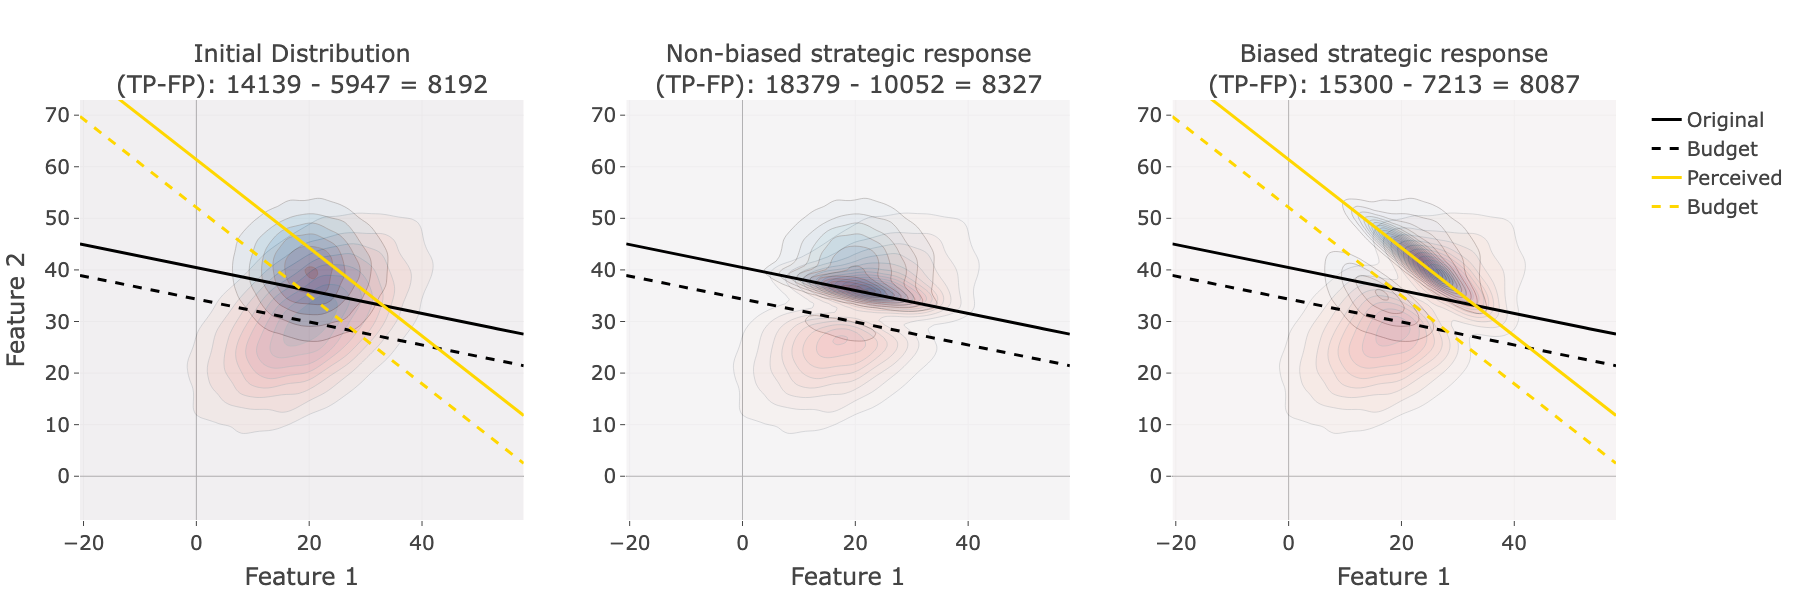
\includegraphics[width=0.9\linewidth]{Figures/1_all_three_GOATEDPLOT1_firm_gets_hurt.png}
    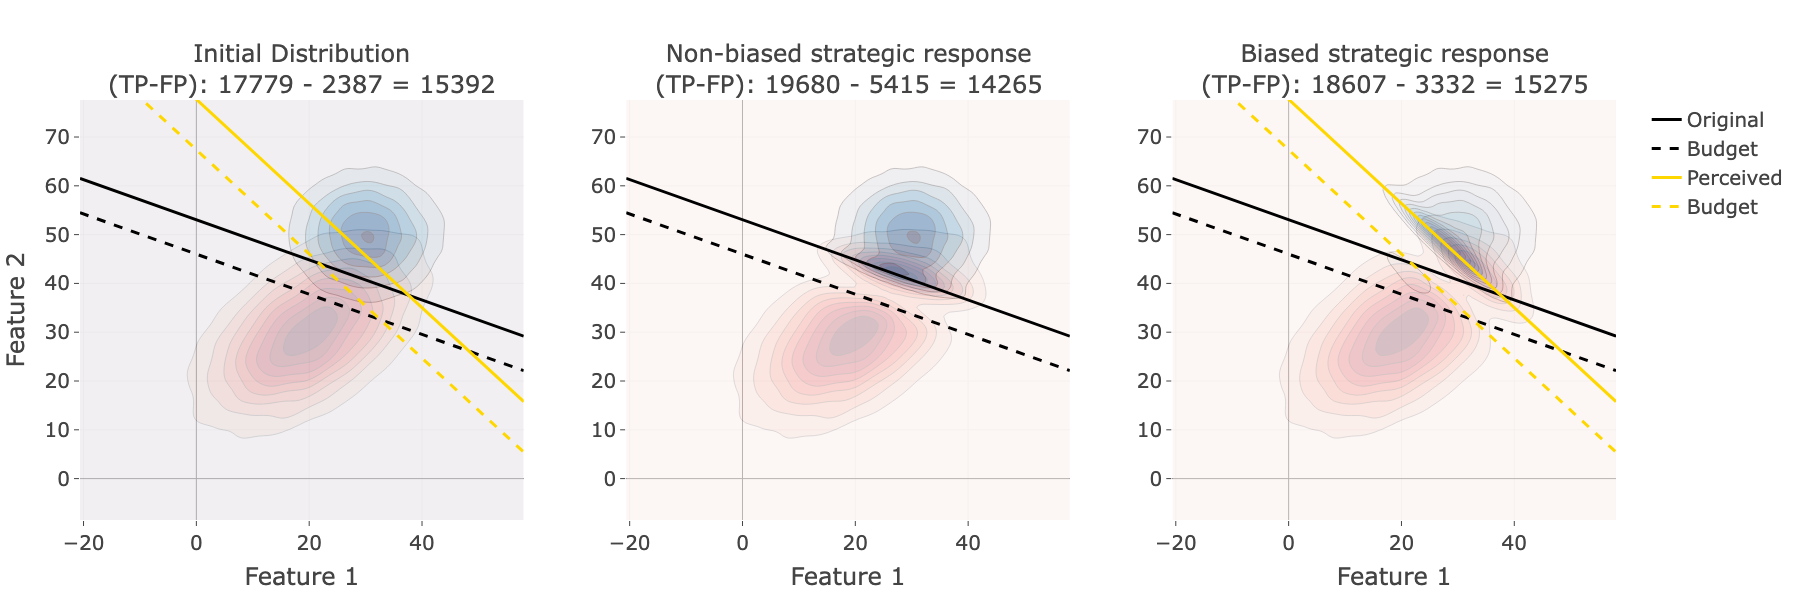
\includegraphics[width=0.9\linewidth]{Figures/1_all_three_GOATEDPLOT2_firm_benefits.png}
    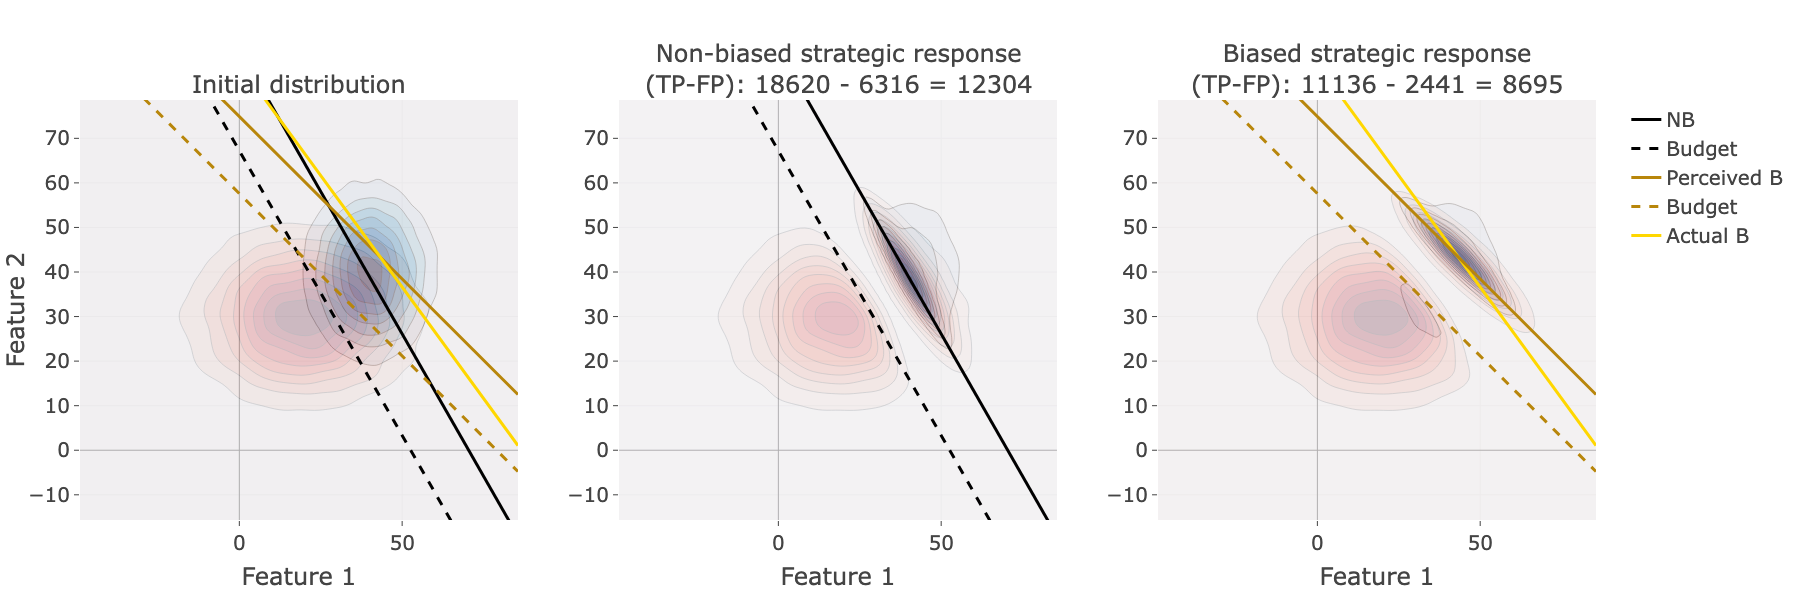
\includegraphics[width=0.9\linewidth]{Figures/1_all_three_GOATEDPLOT_nonoblivious_firm.png}
    \caption{An oblivious firm may have lower (top) or higher (middle) utility when agents are biased (vs. rational). A non-oblivious firm may still have a lower utility when agents are biased (bottom). {The firm's utility is shown above the subplots as (\#TP-\#FP).}}
    \Description[Different scenarios occurring in an example]{An oblivious firm may have lower (top) or higher (middle) utility when agents are biased (vs. rational). A non-oblivious firm may still have a lower utility when agents are biased (bottom).}
    \label{fig:firm-benefit-hurt-dist}
\end{figure*}

We start with the baselines (an oblivious firm that keeps the classifier fixed). In the top row scenario, the firm is negatively impacted by agents' behavioral biases, while in the middle row scenario, the firm benefits from agents' biases (both compared to the fully rational setting). The reason for this difference is that there are more qualified agents than unqualified ones who reach the threshold in non-biased responses. On the other hand, under biased responses, there are more unqualified agents who pass the threshold, regardless of their bias (those in region \framebox(7, 9){3} in Fig.~\ref{fig:highlighted}) in the top row scenario. Behavioral responses by these agents negatively impact the firm, as it leads to these qualified agents no longer being accepted. 

Next, we consider the (non-oblivious) firm that adjusts its classifier optimally (accounting for strategic responses \emph{and} behavioral biases, if any). We observe that even though the firm is aware of agents' bias, its loss is higher than the case of rational responses. As seen in the left panel of the bottom row of Figure~\ref{fig:firm-benefit-hurt-dist}, more regions can impact the loss than in Figure~\ref{fig:BR-illustration}. The most important regions in this scenario are the areas accepted by $\vtheta_\text{NB}$ but not by $\vtheta_\text{B}$ (after response), and vice versa. As there are more qualified than unqualified agents in these two regions, the firm is negatively impacted by agents' bias (compared to fully rational agents) even though the firm is aware of the bias.

\end{example}

The next proposition formalizes the above intuition. 

\begin{proposition}\label{prop:mismatch-actual-b} 
    Consider a loss function $l(\vx, (\vtheta, \theta_0))=-u^+\text{TP}+u^-\text{FP}$. Let the pdf of label $y$ agents' feature distribution be $f_y(\vx)$, and the number of label $y$ agents be $\alpha_0$. Let $\mathcal{H}(\vtheta, \theta_0)$ denote the set of agents that satisfy $(1-\sigma(\vtheta))\theta_0\le(\vtheta-\sigma(\vtheta)\vw(\vtheta))^T\vx$, where $\sigma(\vtheta) \coloneqq \frac{\vtheta^T\vw(\vtheta)}{\norm{\vw(\vtheta)}^2}$\footnote{Note that $\sigma(\vtheta)=\frac{\norm{\vtheta}_2}{\norm{\vw(\vtheta)}_2}\cos(\alpha)$ where $\alpha$ is the angle between the actual and perceived decision boundaries. The larger $\alpha$ is, the lower $\sigma(\vtheta)$ is, indicating a more intense bias.}, and the set of agents that attempt to game the algorithm as $\sA(\vtheta, \theta_0) = \{\vx_0: \theta_0 - B \le \vtheta^T\vx_0 < \theta_0 \}$. Denote the set of accepted (resp. rejected) agents by $(\vtheta, \theta_0)$ with $\sY(\vtheta, \theta_0)$ (resp. $\sN(\vtheta, \theta_0)$). Define the sets 
    \begin{align*}        
        &\sS(\vtheta_\text{NB}, \theta_{0, \text{NB}}) \coloneqq \sA(\vtheta_\text{NB}, \theta_{0, \text{NB}})/(\sA(\vtheta_\text{NB}, \theta_{0, \text{NB}})\cap\mathcal{H}(\vtheta_\text{NB}, \theta_{0, \text{NB}})), \\
        &\sT_1=(\sY(\vtheta_\text{NB}, \theta_{0,\text{NB}})\cup \sA(\vtheta_\text{NB}, \theta_{0,\text{NB}}))\cap \sN(\vtheta_\text{B}, \theta_{0,\text{B}})\text{, and} \\
        &\sT_2 = (\mathcal{H}(\vtheta_\text{B}, \theta_{0,\text{B}})\cap \sA(\vw(\vtheta_\text{B}), \theta_{0,\text{B}}))\cup \\
        &\hspace{1cm}((\sY(\vtheta_\text{B}, \theta_{0,\text{B}}) \cap \sN(\vtheta_\text{NB}, \theta_{0,\text{NB}}))/\sA(\vtheta_\text{NB}, \theta_{0,\text{NB}})).
    \end{align*}
    Then:\\[2pt]
    \hspace*{0.1in}{\textbf{(a)}} If $\int_{x\in \sS(\vtheta_\text{NB}, \theta_{0, \text{NB}})} u^- f_0(\vx)\alpha_0 d\vx \le \int_{x\in \sS(\vtheta_\text{NB}, \theta_{0, \text{NB}})} u^+ f_1(\vx)\alpha_1 d\vx $ we can say: 
    \begin{align}\label{eq:firm-loss-comp-benefit}
        \sL(\vw(\vtheta_\text{B}), (\vtheta_\text{B}, \theta_{0, \text{B}}))&\le \sL(\vw(\vtheta_\text{NB}), (\vtheta_\text{NB}, \theta_{0, \text{NB}}))\notag \\
        &\le \sL(\vtheta_\text{NB}, (\vtheta_\text{NB}, \theta_{0, \text{NB}}))
    \end{align}
    \hspace*{0.1in}{\textbf{(b)}} If $\int_{x\in \sS(\vtheta_\text{NB}, \theta_{0, \text{NB}})} u^+ f_1(\vx)\alpha_1 d\vx \le \int_{x\in \sS(\vtheta_\text{NB}, \theta_{0, \text{NB}})} u^- f_0(\vx)\alpha_0 d\vx $ we can say: 
    \begin{align}\label{eq:firm-loss-comp-hurt}
        \max\{\sL(\vtheta_\text{NB}, (\vtheta_\text{NB}, \theta_{0, \text{NB}}))&,\; \sL(\vw(\vtheta_\text{B}), (\vtheta_\text{B}, \theta_{0, \text{B}}))\}\notag\\
        &\le \sL(\vw(\vtheta_\text{NB}), (\vtheta_\text{NB}, \theta_{0, \text{NB}}))
    \end{align}
    \hspace*{0.1in}{\textbf{(c)}} If $\int_{\vx\in\sT_1}(-u^+f_1(\vx)\alpha_1+u^-f_0(\vx)\alpha_0)d\vx \le \int_{\vx\in\sT_2}(-u^+f_1(\vx)\alpha_1+u^-f_0(\vx)\alpha_0)d\vx$ we can say:
    \begin{align}\label{eq:firm-loss-comp-hurt-NB-B}
        \sL(\vtheta_\text{NB}, (\vtheta_\text{NB}, \theta_{0, \text{NB}}))&\le \sL(\vw(\vtheta_\text{B}), (\vtheta_\text{B}, \theta_{0, \text{B}}))\notag\\
        &\le \sL(\vw(\vtheta_\text{NB}), (\vtheta_\text{NB}, \theta_{0, \text{NB}}))
    \end{align}
\end{proposition}
Part (a) states that if a firm is unaware of agents' behavioral biases, it will suffer a lower loss when the population is biased compared to fully rational. This is the intuitively expected scenario (behaviorally biased agents are less adept than fully rational ones at gaming the algorithm). On the other hand, statement (b) reflects the less expected outcome: a firm unaware of behavioral biases will have \emph{lower} utility when agents are biased compared to if they had been fully rational (as more \emph{qualified} than \emph{unqualified} agents undershoot the threshold under this case's condition). Statement (c) further compares the unaware firm with an aware firm and provides a condition where an aware firm's minimal loss is higher than the non-biased minimal loss. This condition relies on the \emph{difference} of qualified and unqualified agents in two regions.
Lastly, we note that even though $\vw(\cdot)$ is not directly seen in the conditions of Proposition~\ref{prop:mismatch-actual-b}, it affects the regions in which the conditions are satisfied. Generally, the influence of weighting functions, such as Prelec function, on $\vtheta$ can be described as $\vw(\vtheta) = \vtheta + \vbeta$ where $\vbeta$ satisfies two conditions: (1) $\sum_i \beta_i = 0$ ensuring that $\sum_i w_i(\vtheta) = 1$ and implying that increasing the perceived importance of one feature necessarily requires under-estimating at least one other feature and (2) $0\le \theta_i + \beta_i \le 1$ ensuring that the adjusted weights remain within the range $[0,1]$. Therefore, the general impact of other forms of $\vw(\cdot)$ will be similar to Prelec function.

\subsection{Impact on Agents' Welfare}\label{sec:agents_welfare}
We end this section by comparing the impacts of behavioral biases on agents' welfare (sum of their utilities). As a baseline, note that if the firm was oblivious to agents' strategic responses and did not adjust the classifier, agents would have lower welfare when they are behaviorally biased (compared to when rational). This is an expected outcome since behaviorally biased agents are worse at gaming the algorithm and respond sub-optimally. But, perhaps more unexpectedly, when the firm adjusts its classifier in response to agents' strategic behavior and behavioral biases, various scenarios can occur, in some of which behavioral agents obtain \emph{higher} welfare than if they had been rational. For instance, in the bottom row of Figure~\ref{fig:firm-benefit-hurt-dist}, qualified agents have \emph{higher} social welfare when they are behaviorally biased compared to if they had been rational. We provide additional intuition for reasons for this in a 2-D feature space example below. %in Appendix~\ref{app:welfare}. 

Figure~\ref{fig:SW-regions} highlights the change in utility when agents are behaviorally biased (vs. when they were rational) across different regions in the feature space, with the regions generated based on the firm's optimal choice of threshold and agents' responses to it. In particular, the utility of agents in the green-highlighted region (this is $\sY(\vtheta_\text{B}, \theta_{0,\text{B}}) \cap \sN(\vtheta_\text{NB}, \theta_{0,\text{NB}})$ in Proposition~\ref{prop:mismatch-actual-b}) increases when they are behaviorally biased. One subset of agents in this region are those 
%$\sY(\vtheta_\text{B}, \theta_{0,\text{B}}) \cap \sN(\vtheta_\text{NB}, \theta_{0,\text{NB}})\cap \sA(\vtheta_\text{NB}, \theta_{0, \text{NB}})$ where 
who in the rational case exert effort to get admitted and have a utility $r-c(\vx,\vx_0)$, whereas in the behaviorally biased case they attain utility $r > r-c(\vx,\vx_0)$ as they get admitted without any effort (and they correctly assume so). Another one is %subset is $(\sY(\vtheta_\text{B}, \theta_{0,\text{B}}) \cap \sN(\vtheta_\text{NB}, \theta_{0,\text{NB}}))/\sA(\vtheta_\text{NB}, \theta_{0,\text{NB}})$ which is 
the subset of agents who would not try to get to the decision boundary in the rational case (and so have utility of $0$), but in the behavioral case, they are receiving utility $r$ without any movement and due to the change of the decision boundary. For the numerical example in the bottom row of Figure~\ref{fig:firm-benefit-hurt-dist}, there are more agents in this green-highlighted region than in the remaining red-highlighted regions (where biased agents have lower utility than rational agents), leading to an overall higher welfare for all agents when they are biased compared to when they were rational. 

\begin{figure}[ht]
    \centering
    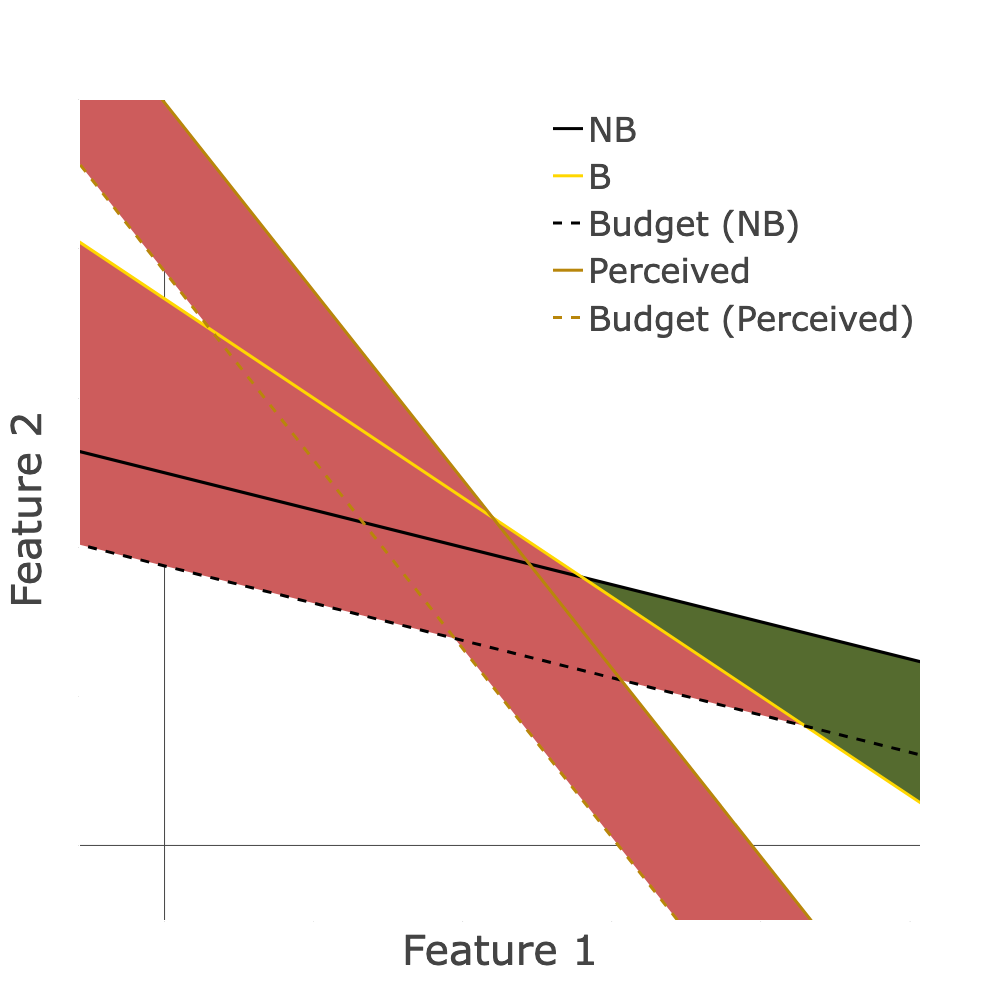
\includegraphics[width=0.6\linewidth]{Figures/SW_highlighted regions.png}
    \caption{Regions where agents have higher (green) or lower (red) utility when biased vs. had they been fully rational.}
    \Description[Welfare regions]{Regions where agents have higher (green) or lower (red) utility when biased vs. had they been fully rational.}
    \label{fig:SW-regions}
\end{figure}


%For B responses, the social welfare for qualified and unqualified agents drops, while unqualified agents get hurt more because they have a higher than necessary or unnecessary cost. 

% Figure~\ref{fig:SW-regions} highlights the change in utility when agents are behaviorally biased (vs. when they were rational) across different regions in the feature space, with the regions generated based on the firm's optimal choice of threshold and agents' responses to it. In particular, the utility of agents in the green-highlighted region (this is $\sY(\vtheta_\text{B}, \theta_{0,\text{B}}) \cap \sN(\vtheta_\text{NB}, \theta_{0,\text{NB}})$ in Proposition~\ref{prop:mismatch-actual-b}) increases when they are behaviorally biased. One subset of agents in this region are those 
% %$\sY(\vtheta_\text{B}, \theta_{0,\text{B}}) \cap \sN(\vtheta_\text{NB}, \theta_{0,\text{NB}})\cap \sA(\vtheta_\text{NB}, \theta_{0, \text{NB}})$ where 
% who in the rational case exert effort to get admitted and have a utility $r-c(\vx,\vx_0)$, whereas in the behaviorally biased case they attain utility $r > r-c(\vx,\vx_0)$ as they get admitted without any effort (and they correctly assume so). Another one is %subset is $(\sY(\vtheta_\text{B}, \theta_{0,\text{B}}) \cap \sN(\vtheta_\text{NB}, \theta_{0,\text{NB}}))/\sA(\vtheta_\text{NB}, \theta_{0,\text{NB}})$ which is 
% the subset of agents who would not try to get to the decision boundary in the rational case (and so have utility of $0$), but in the behavioral case, they are receiving utility $r$ without any movement and due to the change of the decision boundary. For the numerical example in the bottom row of Figure~\ref{fig:firm-benefit-hurt-dist}, there are more agents in this green-highlighted region than in the remaining red-highlighted regions (where biased agents have lower utility than rational agents), leading to an overall higher welfare for all agents when they are biased compared to when they were rational. 

% \begin{figure}[ht]
%     \centering
%     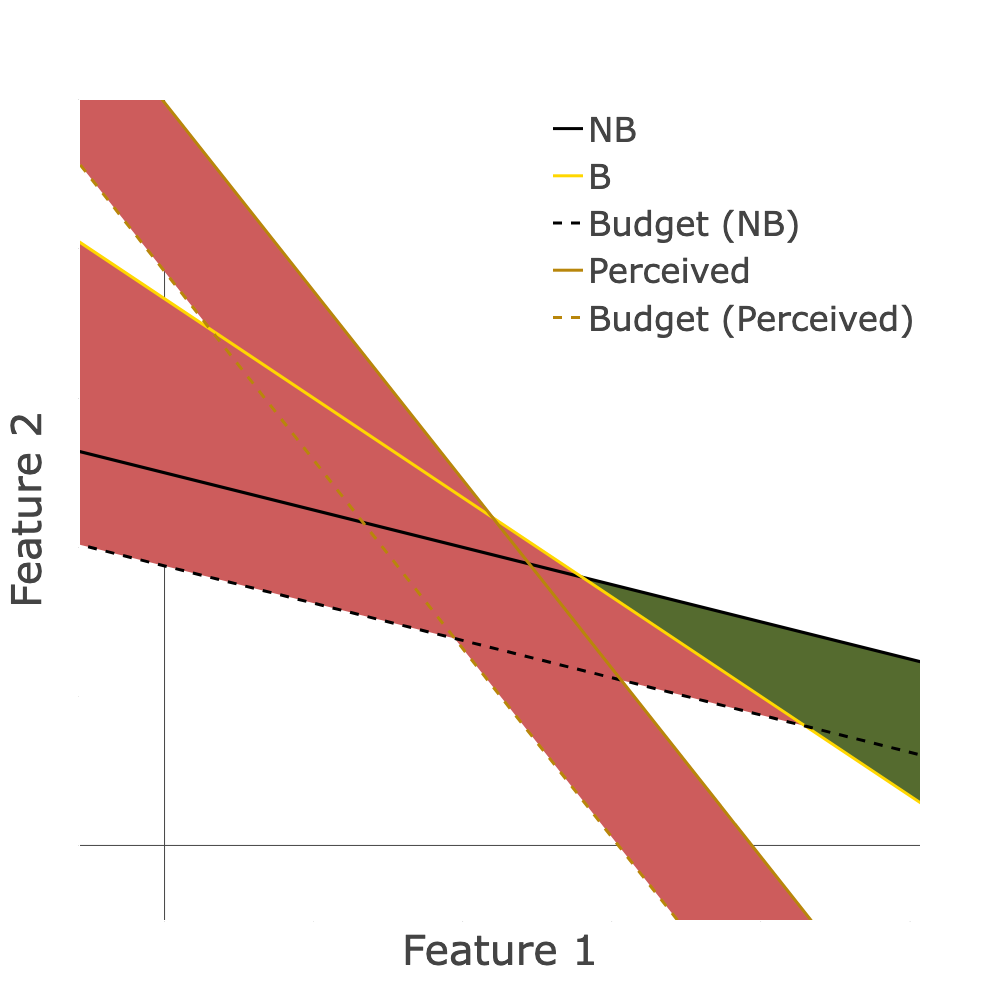
\includegraphics[width=0.5\linewidth]{Figures/SW_highlighted regions.png}
%     \caption{Regions where agents have higher (green) or lower (red) utility when biased vs. when rational.}
%     \label{fig:SW-regions}
% \end{figure}

%In the behavioral case, most regions will not have higher social welfare (Figure~\ref{fig:SW-regions}). Intuitively, for the B case, a firm will ``tilt'' the NB decision boundary to automatically accept more qualified agents and reject more unqualified agents. By this intuition, the firm will see mostly qualified agents in the green region in Figure~\ref{fig:SW-regions} and mostly unqualified agents in the red regions in Figure~\ref{fig:SW-regions}. 
